% Users can also go through the FAQs available on the journal's submission webpage.
%
% Steps to compile: latex, bibtex, latex latex
%
% For tracking purposes => this is v1.3 - May 2012


\documentclass{acmlarge-edm}

% Metadata Information
\acmVolume{1}
\acmNumber{2}
\acmArticle{3}
\acmYear{2012}
\acmMonth{5}  % can also put in literal name

\usepackage{graphics}

% Metadata Information would go here

% Document starts
\begin{document}


% Title portion
\title{Measuring the Moment of Learning}
\author{Brett van de Sande
\affil{Arizona State University\\bvds@asu.edu}}

%
%  Cool LaTeX resource:
%   http://en.wikibooks.org/wiki/LaTeX

\begin{abstract}
We introduce a method to determine the probability that an individual 
student has learned a particular skill at some moment of time. 

The method involves applying a model of learning
we investigate three 
models of student learning 
determining when an individual student has learned a particular skill.
We use the Akaike Information Criterion to investigate the three
models in the context of students using an Intelligent Tutoring System.  
We introduce a multi-model approach for determining 
the probability that a student has learned a given skill at a 
particular problem-solving step.  We then investigate how well this
approach works when applied to student data.  We show that, although the
associated errors are large, our method can detect significant learning. 
\end{abstract}

\keywords{data mining, models of student learning}

\begin{bottomstuff}
Funding for this research was provided by the Pittsburgh Science of
Learning Center which is funded by the National Science Foundation
award No. SBE-0836012.
\end{bottomstuff}


\maketitle


\section{Introduction}

%
%  There is a post-it with note''  ``ICAP frame chi Cog Sci''
%  http://gamesandimpact.org/uncategorized/cgi-qa-with-asu-fellow-dr-michelene-micki-chi/
%

%Talk about ultimate goal of using this to determine effectiveness
%of help given or of a particular student behavior.

The traditional experimental paradigm for studying student learning
is to use a pre-test and post-test combined with two or more experimental
conditions.  Pre-test and post-test scores can indicate {\em whether}
learning has occurred, but not {\em when} it may have occurred.  
At best, one might infer when learning has occurred if an isolated change to 
the instructional materials or help-giving strategy results in better
post-test performance.  
It is more difficult to infer whether a change in student {\em behavior} at
some point has resulted in greater learning, since student behavior is 
largely uncontrolled and must be recorded in some way.
In a laboratory setting, these issues can be addressed by careful
experimental design, albeit with an accompanying loss of authenticity.

Moving from the laboratory to a more realistic setting, such as a
classroom study, presents as challenge since there is necessarily an
extended time between any pre-test and post-test.  Heckler and 
Sayre~\citeyear{heckler_what_2010} introduce an experimental technique
where they administered a test to a different subgroup of students in
a large physics class each week during the quarter, cycling through
the entire class over the course of the quarter (a
between-students longitudinal study).  With a sufficiently large number
of students (1694 students over five quarters), they were able to produce
plots of student mastery of various skills as a function of time, and
identify exactly which week(s) students learned a particular skill.
However, the shortest time scale that one could imagine for this
kind of approach (administering a test in a classroom setting) can, at
best, be a day or so.  Can we do better?

The use of an intelligent tutor systems (ITS) provides a way forward. 
An ITS is a computer-based learning environment where students
construct problem solutions on a user interface and the system
evaluates the student work at the step-level. 
Examples include the CMU LISP tutor~\cite{corbett_knowledge_1995}, the
Carnegie Learning Cognitive Tutors~\cite{koedinger_illustrating_1998},
and Andes~\cite{vanlehn_andes_2005}.  In these tutors, student
activity is analyzed and logged for each user interface element change, with a granularity
of typically several 10s of seconds.
Instead of relying on a distant pre-test or post-test, the experimenter can examine student
(or tutor system) activity in the immediate vicinity of the event of interest.

Our stated goal is to determine student learning for an individual
student as they progress through a course.  What observable quantities should be used to
determine student mastery?  One possible observable is ``correct/incorrect steps,''  whether 
the student correctly applies a given skill at a particular problem-solving step 
without any preceeding errors or hints.  There are other
observables that may give us clues on mastery: for instance, how much
time a student takes to complete a step that involved a given skill.  However, other such
observables typically need some additional theoretical interpretation. {\em Exempli gratia},
What is the relation between time taken and mastery?  Baker, Goldstein, and
Heffernan~\citeyear{baker_detecting_2011} develop a model of learning
based on a Hidden Markov model approach.  They start with a set of
% BvdS:  use actual number.
25 additional observables (including ``time to
complete a step'') and construct their model and use correct/incorrect steps (as defined above)
to calibrate the additional observables and determine which are significant.

Since correct/incorrect steps is easy to interpret, we will use that
as the starting point for our investigation.  Naturally, it is
desirable to eventually include various other observables in any determination
of student learning.

To start our investigation, we will compare three different models of
learning using data from students taking introductory physics and examine
whether there is empirical support for using one model over the
others.  In fact, using Akaike Information Criteria (AIC), we obtain
results that seem to favor two models over the third, but note
that fitting the models to individual students can make the determination ambiguous.

Second, we introduce a multi-model approach to predict the probability that 
learning has occurred at a given step, and how much
learning has occurred.  We apply our approach to student log data from
and introductory physics course and discuss the reliability of any
predictions of skill mastery.  We find that, for an individual
student and skill, detection of learning has large uncertainties.
However, if one aggregates over skills or students, then learning can
be detected at the desired level of significance.


\subsection{Correct/Incorrect steps}

As mentioned above, we will use correctness/incorrectness of a step to
determine when the student has learned above.  Thus, we need to
define precisely what we mean by a step being correct.

A student attempts some number of {\em steps}  when solving a problem.  
Usually, a step is associated with creating/modifying a single user
interface object (writing an equation, drawing a vector,
defining a quantity, {\em et cetera}) and is a distinct part of the problem solution
(that is, help-giving dialogs are not considered to be steps).
A student may attempt a particular problem solving
step, delete the object, and later attempt that solution step again.
A step is an {\em opportunity} to learn
a given  Knowledge Component (KC)~\cite{vanlehn_behavior_2006} if the student 
must apply that skill to complete the step.

%
%  Not needed in this paper.
%
%Each step $j$ corresponds some some number of student-tutor 
%{\em transactions}: attempts at constructing the associated object, 
%or associated interactions with the Andes help system.  

%Next, we need a model of student learning for a particular KC.
%Since the policies chosen by the random-help version of Andes
%are different for each student,
%we need to determine the point of learning for each student.
For each KC and student, we select all attempted steps that involve application
of that KC and mark each step as ``correct'' if
the student completes that step correctly without any preceeding errors or 
requests for help; otherwise, we mark the step as ``incorrect.''
\label{steps}  % Section reference for correct/incorrect
If each incorrect/correct step is marked with a 0/1, then
a single student's performance on a single KC can be expressed as a bit  sequence,
{\em exempli gratia} 00101011.  We will label
steps with $j\in\left\{1,\ldots,n\right\}$.  

\section{Three models of learning}

\begin{figure}
  \centering 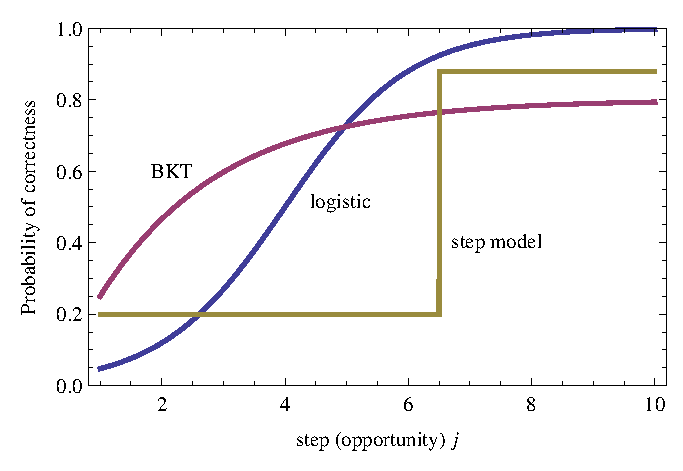
\includegraphics{three-models.eps}
  \caption{Functional form of the three models of student learning.}
    \label{three-models}
\end{figure}


In order to determine when a student has learned a particular still,
we need to introduce a model of learning for that student and skill.
Ideally, the model should have the the following properties:
\label{model-criteria}
%
\begin{enumerate} 

\item Be compatible with actual student behavior.
      That is, its
      functional form should fit well with student data.
      We will explore this question in Section~\ref{model-selection}.  

\item \label{crit:step}
      Give the probability that learning has occurred at a given step.
      We will address this issue in Section~\ref{multi-model}.

\item  \label{crit:perform}
     Assuming learning has occurred at a given step, the model
     should give an prediction for the 
     associated increase in performance and 
     the rate of errors after learning.

\end{enumerate}
%
We will consider three candidate models:  
the Bayesian Knowledge Tracing (BKT) model, the logistic function,
and the ``step model;''
see Fig.~\ref{three-models}.


The first model is the Bayesian Knowledge Tracing (BKT) 
model~\cite{corbett_knowledge_1995}.  The hidden Markov model
form of BKT is often fit to student performance 
data~\cite{beck_identifiability:_2007}.  One can show that
this model, in functional form, is an exponential function
with three model parameters~\cite{van_de_sande_properties_2012}:
%
%  A and \beta are kind of messy, so we don't include them here.
\begin{equation}
         P_\mathrm{BKT}(j) = 1-P(S) -A e^{-\beta j} \; .
\end{equation}
%
One central assumption of BKT is that, given that learning
has not already occurred, mastery is {\em equally probable} on each step.
This assumption of equal probability does not match well with 
our goal of determining empirically the steps where learning has 
actually occurred for an individual student, criterion~\ref{crit:step}.
On the other hand, this model does provide the final
error rate $P(S)$ (the initial error rate is ambiguous), 
so criterion~\ref{crit:perform} is partially satisfied. 

Another model that is frequently used in the context of learning is
the logistic model~\cite{cen_learning_2006,chi_instructional_2011},
%
\begin{equation}
    P_\mathrm{logistic}(j)= \frac{1}{1+\exp\left(-b (j-L)\right)} \; .
\end{equation}
%
It is natural to associate $L$ with the moment of learning.  However,
the finite slope of $P_\mathrm{logistic}(j)$ means that learning may
occur in a range of roughly $1/b$ steps before and after $L$.  For
$P_\mathrm{logistic}(j)$, the gain in performance is always 1 and the
final error rate is always 0.  Thus, although this model makes a
prediction for when the skill is learned, criterion~\ref{crit:step},
it does not predict a gain in performance,
criterion~\ref{crit:perform}.

The third model is the ``step model'' which assumes that learning 
occurs all at once; this corresponds to the ``eureka learning''
discusse by \cite{baker_detecting_2011}.  It is defined as:
%
\begin{equation}
    P_\mathrm{step}(j)= \left\{\begin{array}{cc}
                 g, & j<l \\
                 1-s, & j\ge L 
                 \end{array} \right. 
\end{equation}
%
where $L$ is the step where the student first shows mastery of the KC,
$g$ is the ``guess rate,'' the probability that the student gets a
step correct by accident, and $s$ is the ``slip rate,'' the chance
that the student makes an error after learning the skill.  These are
analogous to the guess and slip parameters of
BKT~\cite{corbett_knowledge_1995}.  The associated gain in performance
is $1-g-s$ and the error rate after learning is simply $s$ in this
model.  Thus, this model satisfies criteria \ref{crit:step} and
\ref{crit:perform}.

\section{Model selection using AIC}
\label{model-selection}

The BKT and logistic function models are widely used and
we have introduced the step model $P_\mathrm{step}(j)$
as an alternative.  How
well do these models match actual student behavior?
Since we will use the step model in subsequent
work, it would be reassuring to know whether it describes the student data as 
well (or better than) the other two models.  We will use the Akaike Information Criterion (AIC) for this purpose~\cite{akaike_new_1974,burnham_model_2002}.
AIC is defined as
%
\begin{equation}
   \mathrm{AIC}= -2 \log\left(\mathcal{L}\right) + 2K
\end{equation}
% 
where $\mathcal{L}$ is the maximized value of the likelihood function
and $K$ is the number of parameters in the model.
 AIC is an estimate of the expected relative ``distance''
between a given model and the true model (assumed to be complicated) 
that actually generated the observed data.  It is valid in limit of 
many data points, $n\to\infty$, with leading corrections of order $1/n$.

A related method for choosing between models is the Bayesian
Information Criterion (BIC) introduced by
Schwarz~\citeyear{schwarz_estimating_1978}.  BIC is defined as
%
\begin{equation}
   \mathrm{AIC}= -2 \log\left(\mathcal{L}\right) + K \log\left(n\right)
\end{equation}
% 
where $n$ is the number of data points.
Burnham \& Anderson~\citeyear[Sections~6.3 \& 6.4]{burnham_model_2002} explain
that BIC is more appropriate in cases where the ``true'' model that
actually created the data is relatively simple (few parameters).  If
the true model is contained in the set of models being considered,
then BIC will correctly identify the true model in the $n\to\infty$
limit.  For BIC to have this property, the true model must stay fixed as 
$n$ increases.  
The authors argue that, while BIC may be appropriate in some
of the physical sciences and engineering, in the biological and social
sciences, medicine, and other ``noisy'' sciences, the assumptions that
underlie BIC are generally not met.  In particular, as the sample size
increases, it is typical that the underlying ``true'' model also
becomes more complicated.  This is certainly true in educational
datamining: datasets are increased by adding data from new schools, or
different years and one generally expects noticeable variation of student
behavior from school to school or from year to year.  In such cases, one
safely can say that the ``true'' model is complicated (because people are
complicated) and becomes more complicated as a dataset is increased in
size.  Although most authors quote both AIC and BIC values, there
is good reason to believe that AIC is generally more appropriate for
educational datamining work.

\subsection{Method}


\begin{figure}
  \centering 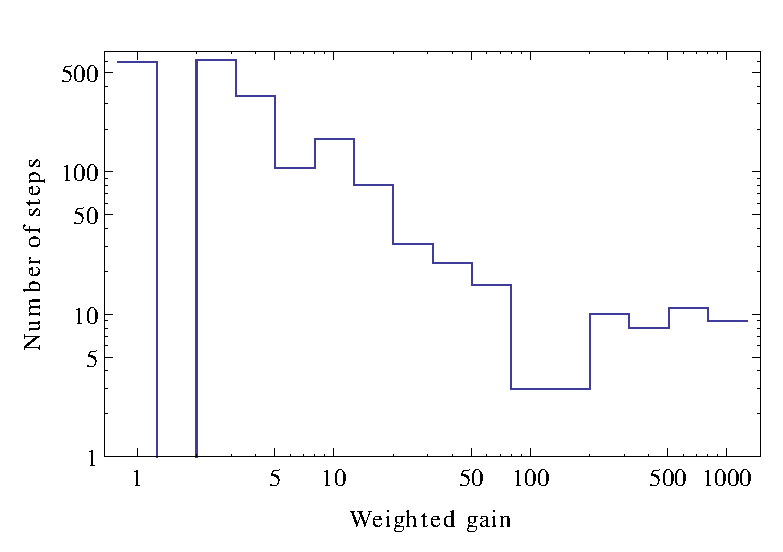
\includegraphics{student-kc-length-histogram.eps}
  \caption{Histogram of number of distinct student-KC sequences in student 
    dataset $\mathcal{A}$ having a given number of steps $n$.}
    \label{student-length-histogram}
\end{figure}

We examined log data from 12 students taking an intensive introductory
physics course at St.\ Anselm College during summer 2011.  The course
covered the same content as a normal two-semester introductory course.
Log data was recorded as students solved homework problems while using
the Andes intelligent tutor homework system.  231 hours of log data
were recorded.
%, covering 85,744 transactions, and 26,204 student steps.  
Each step was assigned to one or more different KC's.  The dataset
contains a total of 2017 distinct student-KC sequences covering a total of
245 distinct KC's.  We will refer to this dataset as student dataset
$\mathcal{A}$.  See Figure~\ref{student-length-histogram} for a
histogram of the number student-KC sequences having a given number of
steps.

Most KC's are associated with physics
or relevant math skills while others are associated with 
Andes conventions or user-interface actions (such as, notation
for defining a variable).  The student-KC sequences with the largest 
number of steps are associated with user-interface related skills,
since these skills are exercised throughout the entire course. 

One of the most remarkable properties of the distribution in
Fig.~\ref{student-length-histogram} is the large number of
student-KC sequences containing just a few steps.
The presence of many student-KC sequences with just one or two
steps may indicate that the default cognitive model associated 
with this tutor system may be sub-optimal; to date, there has not 
been any attempt, to date, to improve on the cognitive model of 
Andes with, say, Learning Factors Analysis~\cite{cen_learning_2006}.
Another contributing factor is the way that introductory physics is 
taught in most institutions, with relatively little repetition of 
similar problems.  This is quite different than, for instance, 
a typical middle school math curriculum where there are a large number
of similar problems in a homework assignment.

\subsection{Analysis}

\begin{figure}
  \centering 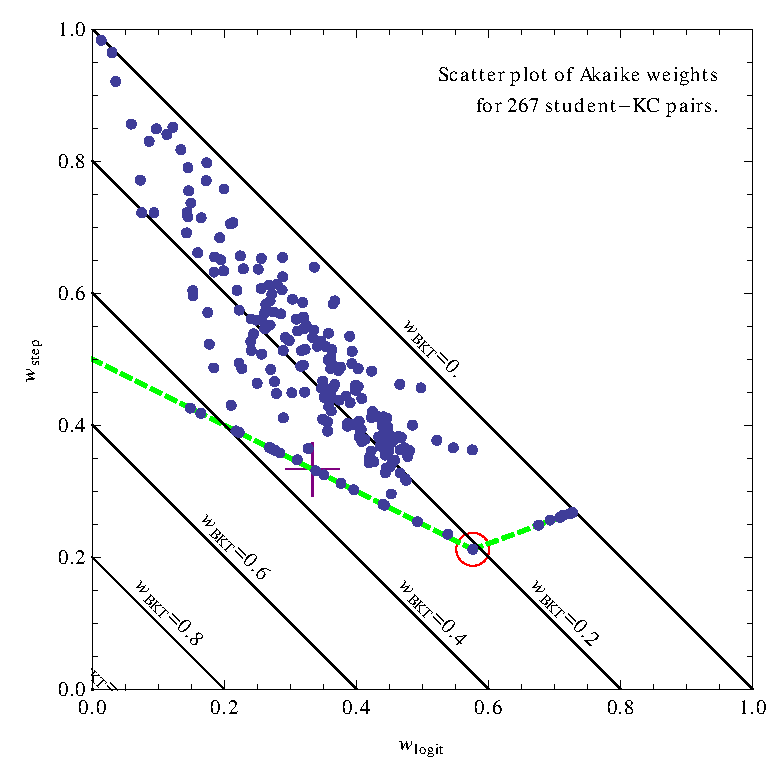
\includegraphics{scatter-weights.eps}
  \caption{Scatter plot of  Akaike weights for the three models, 
   $P_\mathrm{step}$, $P_\mathrm{logistic}$, and $P_\mathrm{BKT}$, 
   when fit to student-KC sequences from an introductory physics course.
   The point where all models are equal,
   $w_\mathrm{step}=w_\mathrm{logistic}=w_\mathrm{BKT}=1/3$, is
   marked with the lower cross.  
   The average of the  weights is marked with
   the upper cross.
  The dashed line on the left represents points
   where $w_\mathrm{step}=w_\mathrm{BKT}$.  Finally, the dashed line on 
   the right marks data with bit sequences of the form
   $00\cdots 011\cdots 1$.} 
   \label{scatter1}
\end{figure}

Since the goodness of fit criterion, AIC, is valid in the limit of
many steps, we include in this analysis only student-KC sequences that
contain 10 or more steps, reducing the number of student-KC sequences to
267, covering 38 distinct KC's.  We determine the correctness of each
step (Section~\ref{steps}), constructing a bit sequence, {\em exempli
gratia} 001001101, for each student-KC sequence.  This bit sequence is then
fit to each of the three models, $P_\mathrm{step}$,
$P_\mathrm{logistic}$, and $P_\mathrm{BKT}$ by maximizing the
associated log likelihood.
%This determines the free parameters in each model. 
We then calculate the AIC score for each fit.  
Finally, we calculated the Akaike weights, $w_\mathrm{logistic}$, $w_\mathrm{step}$, and $w_\mathrm{BKT}$ for each student-KC sequence~\cite{burnham_model_2002}.
The weights are normalized so that
%
\begin{equation}
   1=w_\mathrm{logistic}+ w_\mathrm{step} + w_\mathrm{BKT} \; .
\end{equation}
%
The Akaike weight represents the relative probability that
a particular model in a given set of models is closest
to the model that has actually generated the data. 

A scatter plot of the weights is shown in Fig.~\ref{scatter1}.
If all three models described the data equally well, then
we would expect points to be scattered evenly about 
center point $w_\mathrm{logistic}= w_\mathrm{step}= w_\mathrm{BKT}=1/3$.
Instead, we see the step model (average weight 0.44) weakly 
favored over the logistic model (average weight 0.37) and 
strongly favored over BKT (average weight 0.18).  Indeed, we 
find no data points where $w_\mathrm{step}< w_\mathrm{BKT}$,
although there is a noticeable accumulation of points along the line 
$w_\mathrm{step}= w_\mathrm{BKT}$.

Note that data in the form of incorrect steps then correct steps, 
{\it exempli gratia} $00\cdots 011\cdots 1$,
is fit perfectly by both the $P_\mathrm{step}$ and 
$P_\mathrm{logistic}$ models.  
In this case, since $P_\mathrm{logistic}$ has one fewer parameter
than $P_\mathrm{step}$, it is favored by AIC by a constant factor and
$w_\mathrm{step}=\mathrm{e}^{-1} w_\mathrm{logistic}$.  This case is
plotted as the increasing dashed line in Fig.~\ref{scatter1}.

Since the student-KC sequences contain an average of about $n=16$ 
steps, it is surprising that we find that AIC so strongly
discriminates between the models.  Perhaps this is due to
some finite $n$ correction?  Recall that AIC is only 
strictly valid in the $n\to\infty$ limit.

\subsection{Random data}


\begin{figure}
  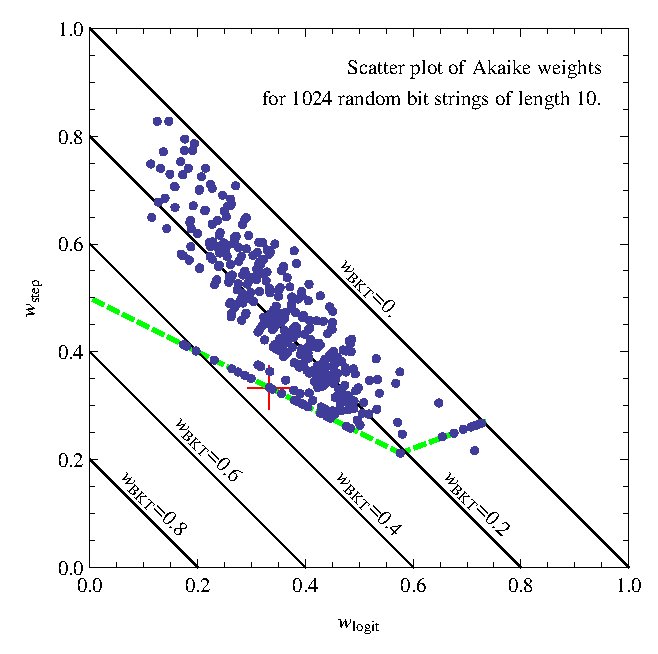
\includegraphics{scatter10.eps} \hfill
  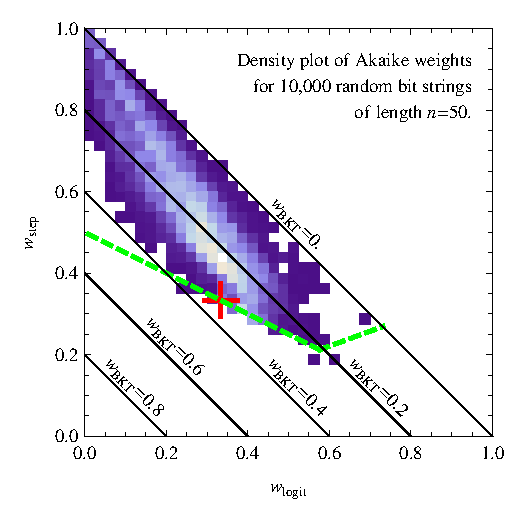
\includegraphics{density50.eps}
  \caption{Akaike weights for the three models, 
   $P_\mathrm{step}$, $P_\mathrm{logistic}$, and $P_\mathrm{BKT}$, 
   when fit to randomly generated data.  The point where
   $w_\mathrm{step}=w_\mathrm{logistic}=w_\mathrm{BKT}=1/3$ is
   marked with a cross.  For these datasets, each 
   model should perform equally well, since, with an appropriate
   choice of parameters, they all can be made equal to 
   the model that was used to generate the data.}\label{scatter2}
\end{figure}

To further investigate this situation, we constructed an
artificial dataset containing random bit sequences (each
step has 50\% probability of being ``correct'') of length 
$n\in\left\{10,20,30,40,50\right\}$.
This dataset corresponds to a model of the form
%
\begin{equation}
        P_\mathrm{random}(j)=1/2 \; .
\end{equation}
%
We then repeated our analysis of the three models using this dataset
and AIC as our selection criterion.  Note that all three models,
with a suitable choice of parameters, can be made equal to 
$P_\mathrm{random}$.

As mentioned earlier, for data that is generated by a simple 
model ($P_\mathrm{random}$ is about as
simple as one can get) and the ``true'' model is included among
the set of models, BIC is the more appropriate criterion
for model selection~\cite[Sections~6.3 \& 6.4]{burnham_model_2002}.
However, the only difference between AIC and BIC for our results is that BIC favors
$P_\mathrm{logistic}$ more strongly over $P_\mathrm{step}$ and
$P_\mathrm{BKT}$.  Thus, using BIC would shift the weights so that
$w_\mathrm{logistic}$ would increase somewhat over the other two
weights.  However, in order to maintain consistency with
our experimental results, we used AIC for the random data as well;
see Fig.~\ref{scatter1}.  This use of AIC versus BIC does not 
affect our conclusions.

For data generated by $P_\mathrm{random}$,
one expects that all three models should perform equally
well since all three can equal (with suitable choice of parameters)
the known correct model $P_\mathrm{random}$.  Thus, we would expect
a scatter plot of the Akaike weights to center around
$w_\mathrm{logistic}=w_\mathrm{step}=w_\mathrm{BKT}=1/3$.  Instead, we
find that $P_\mathrm{step}$ is highly favored over the other two; see
Fig.~\ref{scatter2}. This bias seems to persist as we increase $n$.

\begin{figure}
   \centering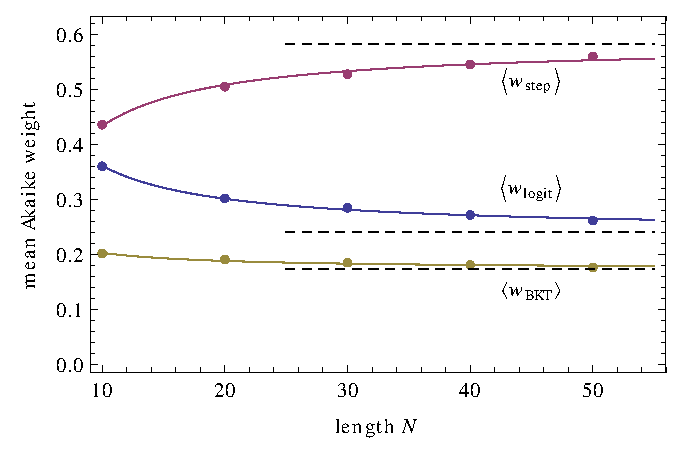
\includegraphics{mean-weights.eps}
  \caption{Mean Akaike weights for the three models, 
   $P_\mathrm{step}$, $P_\mathrm{logistic}$, and $P_\mathrm{BKT}$, 
   when fit to randomly generated data of length $n$.
   (Each mean is calculated by averaging over 10,000 random bit sequences.)
   Also shown is a fit to a function of the form $a+b/n$ and
   a dashed line marking the asymptotic value $a$.
   Note that the differences between the weights persist
   in the $n\to\infty$ limit.}\label{meanweight}
\end{figure}

If we plot the average weight as a function of $n$, we find
that the differences between the weights persist
in the $n\to\infty$ limit;  see Fig.~\ref{meanweight}.
If we fit the average weights to a constant plus $1/n$;
the fits are:
%
\begin{eqnarray}
 \langle w_\mathrm{step}\rangle &=& 0.58 - \frac{1.50}{n} \\
 \langle w_\mathrm{logistic}\rangle &=& 0.24 + \frac{1.2}{n} \\
 \langle w_\mathrm{BKT}\rangle &=& 0.17+\frac{0.30}{n} \; .
\end{eqnarray}
%
This shows that AIC, in the asymptotic limit $n\to\infty$, 
still favors  $P_\mathrm{step}$ over the other two models
when used to evaluate randomly generated data.

If we repeat this analysis with BIC, we would also
find that the weights converge to a constant value with 
$1/n$ leading errors.  The only difference is that the logistic
model has a larger weight than the other two.  This is to be
expected since all three models contain the true model.

\subsection{Summary}

In conclusion, we obtain some surprising results when we compare
the three models,  $P_\mathrm{step}$, $P_\mathrm{logistic}$, and
$P_\mathrm{BKT}$, using individual student data.   We see that AIC
weakly favors the step model over the logistic model in a fashion that one might expect.
However, in an unexpected fashion, we see that both are favored
strongly over the BKT model.  We see that this effect remains for
randomly generated data and is not a finite $n$ effect.

In particular, for any bit sequence,  $P_\mathrm{BKT}$ {\em never}
fits the data better than $P_\mathrm{BKT}$.  Since 
both models have three parameters, this result holds for any maximum
likelihood-based criterion, including both AIC and BIC.  We don't have
an analytic proof for this result, 
but the numerical evidence (see Fig.~\ref{meanweight}) is quite strong.
In other words, even if I use $P_\mathrm{BKT}$ (for some set of model parameters) 
to generate a bit sequence, I can
always adjust the parameters in $P_\mathrm{step}$ so that it
fits the bit sequence as well as, or better than, $P_\mathrm{BKT}$.


% How can we understand this?  Each model can be thought of as a
% set of functions.  One can ask how well each set of functions spans
% the space of all possible functions.  Evidently, the step model spans
% the space of all possible functions much better than the BKT model
% does.    Imagine that I choose some values for the parameters
% of the BKT model and then use the BKT model to construct a
% bit sequence $01011011\ldots$.  The 



What does this mean?  Let us think
more carefully about maximum liklihood.
If I use a model to generate a single bit sequence, I cannot tell from
that sequence the exact probability function (the probability as a
function of $j$) that generated it.  At best, I can only
talk about probability functions that {\em may} have generated that sequence.
On the other hand, if I use a probability function to generate a collection of infinitely many
sequences, then I know the exact probability for each step and, therefore, the exact function that
produced those probabilities.  If that function comes from a
particular model $\mathcal{A}$ (for some choice of model parameters),
 then I can saftely conclude that model $\mathcal{A}$ is the correct model.

Thus, when we are fitting individual student data to a model (fitting
model parameters separately for each student), then we can make no
statements about what model is ``correct'' in the sense that it may
have generated the data.  We can only talk about a model being a good
fit in the sense that it is ``close'' to the data.
On the othe hand, if we aggregate data from many students and fit to a
model (finding the best fit model parameters), then we can talk about
a model being correct in the usual sense  that it may have generated
the data.

In the present work, we are more concerned about being ``close'' to
the student data than finding the correct theory of learning, so the
fact that the step model fits the data better than the logistic function and
the BKT model is good news.  However, one should not then conclude
that the step function is a better model of student learning.

Finally, we see that the scatter plot of Akaike weights for student
data is remarkably similar to the scatter plots for the random model.
This suggests that the student data has a high degree of randomness,
and, in general, that study of the random model may be quite useful for better
understanding the student data.

% However, our use of the step model is primarily motivated
% by criteria~\ref{crit:step} and \ref{crit:perform} of  Section~\ref{model-criteria}.
% In Section~\ref{multi-model}, we show how AIC-based methods
% can yield the probability that learning has occurred during a given step.

\section{Multi-model approach}
\label{multi-model}

We need to determine the step where a specific student has learned a
particular skill.  Our strategy is to take the step model, 
$P_\mathrm{step}(j)$, and treat $L$ as a constant, yielding a set of $n$ 
sub-models $P_{\mathrm{step},L}(j)$, one for each value of $L$.
We then fit each of the $n$ sub-models to the student data and
calculate an AIC value.  Finally, we find the Akaike weighs for each of the
sub-models.  The Akaike weights give the relative probability that learning
occurred at each step.

\begin{figure}
  \centering 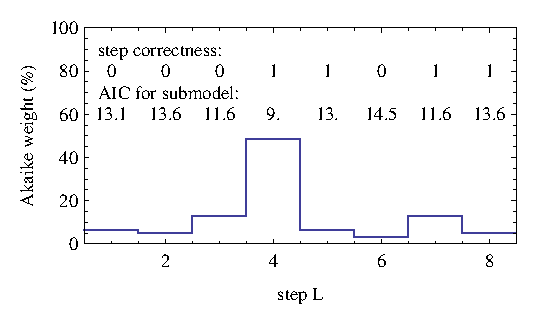
\includegraphics{step-weights.eps}
   \caption{Akaike weights for the submodels $P_\mathrm{step,L}(j)$.  
     This gives the relative probability that
      the student learned the KC just before step $L$.}
    \label{step-weights}
\end{figure}

Let us illustrate this technique with a simple example.  Suppose the
bit sequence for a particular student-KC sequence is 00011011 (8
opportunities); see Fig.~\ref{step-weights}.  We fit this bit sequence to 8
sub-models of the step model, corresponding to $L\in\{1,2,\ldots,8\}$,
by maximizing the log likelihood $\log\mathcal{L}$.  The associated
AIC values are given by $\mathrm{AIC}_L=2 K-\log \mathcal{L}$ where
$K$ is the number of fit parameters.  Note that there are two
parameters ($s$ and $g$) when $L>1$ and there is only one parameter
($s$) when $L=1$.
%
%\begin{table}
%\caption{
%\begin{tabular}{crrrrrrrr}
% opportunity & 1 & 2 & 3 &4 & 5 & 6 & 7 & 8 \\
 % AIC &   13.1 & 13.6 & 11.6 & 9.0 & 13.0 & 14.5 & 11.6 & 13.6 \\
%\end{tabular}
%\end{equation}
%
Not surprisingly, the best fit (lowest AIC) corresponds to the first
``1'' in the bit sequence at step~4.  From the AICs, we calculate 
the Akaike weights
%
\begin{equation}
     w_L=\frac{e^{-\mathrm{AIC}_L/2} }{\sum_{L^\prime}
       e^{-\mathrm{AIC}_{L^\prime}/2}} \; .
\end{equation}
%
The Akaike weight $w_L$ gives the relative probability that sub-model 
$P_{\mathrm{step},L}(j)$ is, of all the sub-models, the closest to the 
the model that actually generated the data.


Note that the case $L=1$ corresponds to the student having 
``learned the skill'' some time before the first step.  That is to say, 
the student does not acquire the skill while using the tutor system.
Thus, $w_1$ should be interpreted as the relative probability
that no learning has occurred while using the tutor system.

\section{Weighted gain}

Our ultimate goal is to distinguish steps that result in 
learning from steps that do not.  Hopefully, one can use this
information to infer something about the effectiveness of the help
given on a particular step, or the effectiveness of
the student activity on that step.

\begin{figure}
  \centering 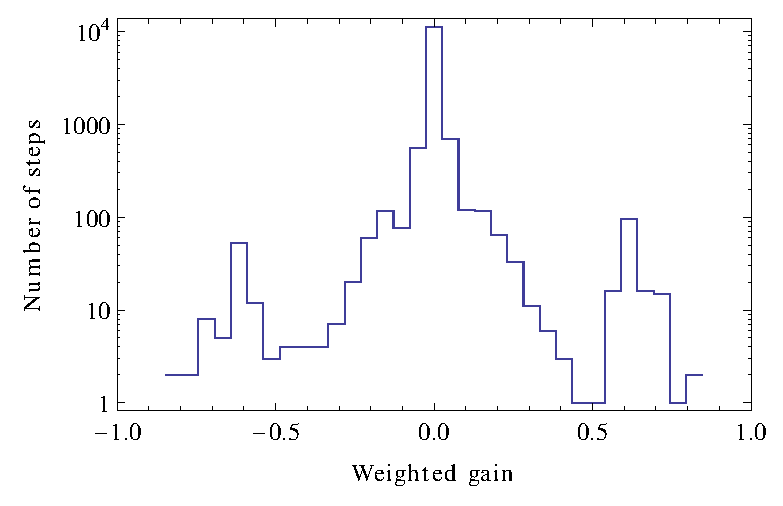
\includegraphics{weighted-gain-histogram.eps}
   \caption{Histogram of weighted gains $w_L \Delta_L$ for
     all steps in all student-KC sequences in student dataset $\mathcal{A}$.}
    \label{weighted-gain-histogram}
\end{figure}

It is not sufficient to know {\it when} learning has occurred but one
must also determine {\it how much} learning has occurred.  Consider
the bit sequence 11011000.  When fit to the step model, the best fit
will occur at $L=6$ but this would correspond to a {\it decrease} in student
performance for that skill.  In many cases seen in our log data, 
the change in student performance is almost zero.  In order to take 
this into account,
we propose using the Akaike weight $w_L$ times the associated learning
gain $\Delta_L$ to characterize a step.  We define the learning gain
$\Delta_L=1-\hat{g}-\hat{s}$ where $\hat{g}$ and $\hat{s}$ are the
Maximum Likelihood estimators for $g$ and $s$ given by submodel
$P_{\mathrm{step},L}(j)$.  For the ``no learning'' case $L=1$, we set
$\Delta_1=0$.  We will call $w_L \Delta_L$ the ``weighted gain''
associated with $P_{\mathrm{step},L}(j)$.  A histogram of $w_L
\Delta_L$ for student dataset $\mathcal{A}$ is shown in
Fig.~\ref{weighted-gain-histogram}.  Note that the vast majority of
steps (29730) have almost zero weighted gain.  We also see that there
is a significant number of steps with negative gain (988), but there
are somewhat more steps with positive gain (1312) .

The fact that there are so many steps with negative gain is
symptomatic of bit sequences that are very noisy (a lot of
randomness).  Indeed, if we compare the histogram for student
dataset $\mathcal{A}$ with the histogram for a randomly 
generated dataset $\mathcal{R}$ (we take $\mathcal{A}$ and
randomly permute the steps) we find a similar distribution;
see Fig.~\ref{weighted-gain-histogram2}.

What would the distribution look like if the data weren't 
so noisy?  To see this, we generated an artificial ``ideal'' dataset
$\mathcal{I}$ where there were no slips or guesses, but having
the same length distribution as $\mathcal{A}$ 
(Fig.~\ref{student-length-histogram}).  Thus, the bit sequences
in $\mathcal{I}$ have the form $00\cdots011\cdots1$.
In this case, for each student-KC sequence, we expect a single 
large weighted gain (corresponding to the first 1 in the bit sequence) 
and the remaining weighted gains to be nearly zero.  The resulting 
distribution of gains is shown
in  Fig.~\ref{weighted-gain-histogram2}.

\begin{figure}
  \centering 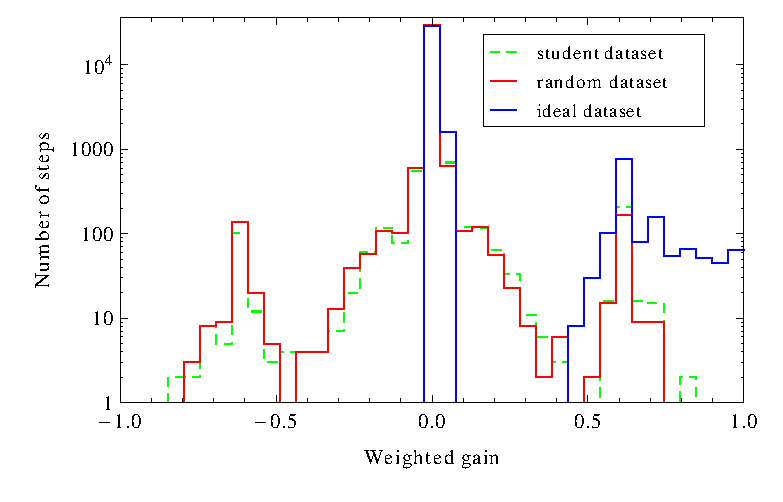
\includegraphics{weighted-gain-histogram2.eps}
   \caption{Histogram of weighted gains $w_L \Delta_L$ for
     the student dataset $\mathcal{A}$, 
     a randomly generated dataset $\mathcal{R}$,
     and an artificial ideal dataset $\mathcal{I}$.}
    \label{weighted-gain-histogram2}
\end{figure}


We propose to use the following average of the weighed gains as
a ``quality index'' for determining how suitable a 
dataset is for determining the point of learning for an individual
student-KC sequence:
%
\begin{equation}
           Q= \frac{1}{N} \sum_\alpha \sum_L w_L \Delta_L
\end{equation}
%
where $\alpha$ is an index running over all student-KC sequences in a 
dataset and $N$ is the number of student-KC sequences.
We use the sample standard deviation of the weighted gains $w_L \Delta_L$
to calculate the standard error associated with $Q$. 

For the random dataset $\mathcal{R}$, the distribution of $\Delta_L$
is symmetric about zero and $Q$ approaches zero as $N \to \infty$.
For the ``ideal'' dataset $\mathcal{I}$, we expect, for the first 1 in
the bit sequence, $w_L$ to be nearly one with the associated $\Delta_L$
also nearly one so that $Q\to 1$ in the limit of many opportunities.
Numerically, we obtain $Q=0.5240\pm0.0003$.  The fact that it is
smaller than one is due to the large number of student-KC sequences having
just a few steps.  For the student dataset $\mathcal{A}$, we obtain
$Q=0.0467\pm0.0065$, which is small, but significant
($p<0.001$). Thus, we conclude that this student dataset is of
sufficient quality to use in determining where learning has occurred.


\section{Conclusion}

We believe that a direct estimate of the moment when a student
learns a skill could be very useful for improving instruction,
improving help-giving and understanding student learning.
However, the question of whether learning has occurred at a particular
step can only be answered in a probabilistic sense:
unambiguous ``Aha moments'' seem to be relatively rare.
Using the Akaike Information Criterion, we have introduced a method
for determining this probability.



As can be seen in
Fig.~\ref{weighted-gain-histogram2}, there is not much difference
between a student dataset and a randomly generated dataset.  However,
the quality index $Q$ which can be used to quantify the
size of the signal as well as the size of the background.  We see that
$Q=0.0467\pm0.0065$ for the student dataset $\mathcal{A}$ is roughly
10\% the size of $Q$ for the ideal dataset $\mathcal{I}$; we interpret
this to mean that the ``signal'' is roughly 10\% as big as the
``noise.''  However, the fact that $Q$ for the student dataset is
seven standard deviations from zero means that we have detected
learning for 2000 student-KC sequences with room to spare.  Using the fact
that the error goes as $1/\sqrt{N}$, where $N$ is the number 
of student-KC sequences, we estimate
that we could still detect learning with only 260 student-KC sequences at the
$p=0.01$ level.  This gives us an initial estimate for the amount of
log data needed to measure the moment of learning, at least for
students using the Andes tutor system.

As seen in Fig.~\ref{student-length-histogram}, we see that many of
the student-KC sequences are quite short.  We speculate that this
is due to to the way that physics is typically taught, with relatively
little reinforcement of specific KCs, emphasizing, instead, more
general problem solving meta-skills.  If we were to repeat this
analysis for high school or grade school math, where there is more
repetition, we speculate that there would be significantly fewer KCs
with less than 10 opportunities and that detecting when learning has
occurred would be significantly easier.


% Bibliography
\bibliographystyle{acmlarge}
\bibliography{education-modeling}



\end{document}
